\section{Method}
\label{sec:method}

% Budget: about 1.0 column-page plus one figure (the model diagram).
% Rubric (3 pts): "clear enough to reproduce, attribution of reused work explicit" (R3).
% Source: distracted_driver.ipynb header (Ablation ladder, Evaluation protocol).

To test whether explicit geometric priors and identity removal reduce driver memorization on unseen subjects, we compare non-neural baselines against a controlled sequence of convolutional models trained under identical driver-disjoint splits.

%-------------------------------------------------------------------------
\subsection{Classical Baselines}
% Source: distracted_driver.ipynb Section 12 (rainforest/hog_random_forest.py features).
To quantify what end-to-end convolutional learning buys over simpler feature pipelines, we evaluate three Random Forest (RF)~\cite{breiman2001rf} baselines (200 unpruned trees with balanced class weights) on the exact same driver-grouped folds and frozen test drivers as our neural models (Sec.~\ref{sec:data}):
\begin{itemize}[leftmargin=*,nosep]
  \item \textbf{HOG + RF (purely non-neural):} Extracts 5,940 Histogram of Oriented Gradients (HOG) features~\cite{dalal2005hog} from each $128 \times 96$ grayscale frame, testing how well hand-crafted appearance gradients generalize to unseen drivers.
  \item \textbf{Pose + RF (image-centered):} Trains an RF on the 19 raw upper-body keypoint coordinates and detection flag from a frozen COCO Keypoint R-CNN~\cite{he2017maskrcnn} (Sec.~\ref{sec:network}).
  \item \textbf{Pose + RF (body-centered):} Uses the same 19 keypoints after translating them to the mid-shoulder origin and scaling by shoulder width, isolating the driver-invariant signal recovered by geometric normalization alone.
\end{itemize}

%-------------------------------------------------------------------------
\subsection{Network Architecture}
\label{sec:network}
% Source: distracted_driver.ipynb Section 4 (DriverNet), table_model_parameters.csv.
\begin{figure*}[t]
  \centering
  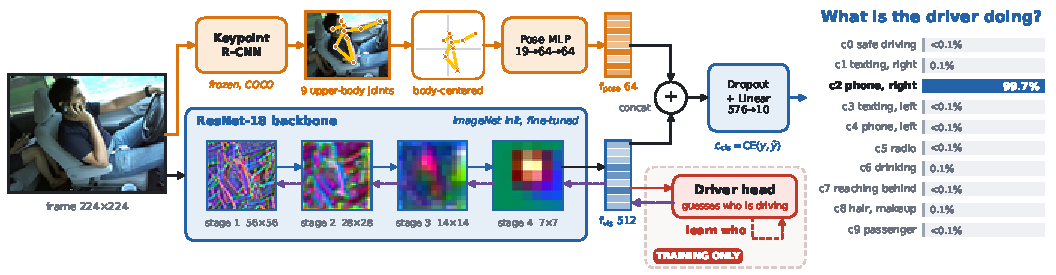
\includegraphics[width=\linewidth]{figures/model.pdf}
  \caption{\textbf{Architecture overview (Configs~\texttt{D-I} and~\texttt{F-I}).}
  A $224 \times 224$ frame passes through a ResNet-18 visual stream (blue) and an optional body-centered pose stream (orange), whose embeddings are concatenated to predict the 10 distraction classes. During training, a driver head attaches to the visual embedding $\mathbf{f}_{\text{vis}}$ to learn driver identity (red dashed arrow) while sending adversarial gradients back into the visual backbone to erase it (purple dashed arrows). See Section~\ref{sec:network} for full details.}
  \label{fig:model}
\end{figure*}


\paragraph{Visual Stream.}
% Source: distracted_driver.ipynb Section 4 (DriverNet), cell 3 settings, table_model_parameters.csv.
We use a ResNet-18~\cite{he2016resnet} backbone operating on $224 \times 224$ ImageNet-normalized RGB frames across four residual stages ($56 \times 56$ to $7 \times 7$). Global average pooling over the final stage yields the visual representation $\mathbf{f}_{\text{vis}} \in \mathbb{R}^{512}$. To test whether pretraining changes how strongly a model memorizes drivers, every configuration is trained both from random initialization (\texttt{-S}) and from ImageNet-1K~\cite{russakovskyImageNet2015} weights (\texttt{-I}).

\paragraph{Body-Centered Pose Stream.}
% Source: distracted_driver.ipynb Section 2 (pose keypoint extraction) and Section 4 (pose MLP).
To supply appearance-free body geometry, we extract 9 upper-body keypoints (nose, ears, shoulders, elbows, and wrists) offline with a frozen COCO Keypoint R-CNN~\cite{he2017maskrcnn} (confidence threshold $0.5$). Raw image coordinates still encode where each driver sits and how large they appear, so we re-express every joint relative to the driver's own shoulders. The origin moves to the midpoint between the shoulders, and one unit equals the shoulder width. Let $\mathbf{k}_j \in [0, 1]^2$ be the image position of joint $j$, with $\mathbf{k}_{\text{ls}}$ and $\mathbf{k}_{\text{rs}}$ the left and right shoulders, respectively, and let $\delta \in \{0, 1\}$ indicate whether a person was detected. With mid-shoulder point $\mathbf{m} = \tfrac{1}{2}(\mathbf{k}_{\text{ls}} + \mathbf{k}_{\text{rs}})$ and shoulder width $w = \max(\|\mathbf{k}_{\text{ls}} - \mathbf{k}_{\text{rs}}\|_2,\, 0.05)$, clamped to avoid dividing by a near-zero width, each joint becomes
\begin{equation}
  \tilde{\mathbf{k}}_j = \delta \, \frac{\mathbf{k}_j - \mathbf{m}}{w},
  \label{eq:pose_norm}
\end{equation}
which is all zeros when no person is detected. Flattening the 9 normalized joints and appending $\delta$ gives a 19-d vector $\mathbf{p} \in \mathbb{R}^{19}$, which a 2-layer Pose MLP ($19 \!\to\! 64 \!\to\! 64$, ReLU) projects to $\mathbf{f}_{\text{pose}} \in \mathbb{R}^{64}$.

\paragraph{Classification Head.}
% Source: distracted_driver.ipynb Section 4 (DriverNet classifier).
The classifier reads $\mathbf{f}_{\text{vis}}$, or $[\mathbf{f}_{\text{vis}};\, \mathbf{f}_{\text{pose}}] \in \mathbb{R}^{576}$ with pose fusion. Dropout ($p = 0.30$) followed by a linear layer outputs class probabilities $\hat{y}$ over the 10 distraction classes, trained with the cross-entropy loss $\mathcal{L}_{\text{cls}} = \mathrm{CE}(y, \hat{y})$, where $\mathrm{CE}(q, p) = -\sum_c q_c \log p_c$ and $y$ is one-hot.

\paragraph{Training-Only Driver Adversary.}
% Source: distracted_driver.ipynb Section 4 (GradReverse, confusion_loss), adversarial_study.ipynb
% Sections 5 and 6 (lambda and ramp, confusion loss).
To remove driver identity from $\mathbf{f}_{\text{vis}}$ at zero test-time cost, we attach a 2-layer MLP driver head $h_d$ ($512 \!\to\! 256 \!\to\! K$, ReLU) during training to predict which of the $K$ training drivers $d$ appears in the frame. Training optimizes two opposing objectives (Fig.~\ref{fig:model}). The head $h_d$ updates only itself to \emph{learn who} is driving by minimizing $\mathrm{CE}(d,\, h_d(\mathbf{f}_{\text{vis}}))$ on detached features, while the backbone updates through a frozen copy of $h_d$ to \emph{hide who} is driving by minimizing one of
\begin{align}
  \mathcal{L}_{\text{GRL}} &= \mathcal{L}_{\text{cls}} - \lambda(p)\,\mathrm{CE}\!\left(d,\, h_d(\mathbf{f}_{\text{vis}})\right),
  \label{eq:grl} \\
  \mathcal{L}_{\text{conf}} &= \mathcal{L}_{\text{cls}} + \lambda(p)\,\mathrm{CE}\!\left(\mathbf{u},\, h_d(\mathbf{f}_{\text{vis}})\right),
  \label{eq:conf}
\end{align}
where $\mathbf{u} \in \mathbb{R}^K$ is the uniform distribution ($1/K$ per driver) and $\lambda(p) = \lambda_{\max}\!\left(\tfrac{2}{1 + \exp(-10p)} - 1\right)$ ramps adversary strength over training progress $p \in [0, 1]$ up to $\lambda_{\max} = 1.0$ via the domain-adversarial (DANN) schedule~\cite{ganin2016dann} (selected in Sec.~\ref{sec:robustness}). Gradient reversal (GRL, Eq.~\ref{eq:grl})~\cite{ganin2016dann} flips the gradient sign so the backbone maximizes driver error; because negative cross-entropy is unbounded, the backbone can cheat by making $h_d$ confidently wrong rather than uncertain. Confusion loss (Eq.~\ref{eq:conf})~\cite{tzeng2015confusion,alvi2018turning} fixes this by pushing $h_d$ toward a uniform guess, a bounded target reached only when $\mathbf{f}_{\text{vis}}$ carries no usable driver cues. At each step, $h_d$ chases any remaining identity signal while the backbone's adversarial gradient (purple arrows in Fig.~\ref{fig:model}) strips it out across all four ResNet stages.

% Placed where the text has reached page 3's right column, so it floats to the top of
% that column under Fig. 1.
\begin{table}[t]
  \centering
  \small
  \caption{\textbf{Model ablation ladder.} Every row is trained both from
  scratch (\texttt{-S}) and from ImageNet-1K weights (\texttt{-I}).}
  \label{tab:ablation_ladder}
  \begin{tabular}{@{}llcc@{}}
    \toprule
    ID & Configuration & Driver Adversary & Pose Fusion \\
    \midrule
    \texttt{A} & Baseline & --- & --- \\
    \texttt{B} & + GRL adversary & GRL & --- \\
    \texttt{C} & + Pose fusion & --- & \checkmark \\
    \texttt{D} & Full GRL & GRL & \checkmark \\
    \texttt{E} & + Confusion adversary & Confusion & --- \\
    \texttt{F} & Full Conf. & Confusion & \checkmark \\
    \bottomrule
  \end{tabular}
\end{table}

\paragraph{Ablation Ladder.}
% Source: distracted_driver.ipynb Section 6.2 (configurations).
Our ablation ladder (Table~\ref{tab:ablation_ladder}) is six models that each add or swap one component, trained under both initializations (12 models). Comparing \texttt{B} vs.\ \texttt{E} and \texttt{D} vs.\
\texttt{F} isolates the adversarial objective, while comparing \texttt{D} and
\texttt{F} against \texttt{C} isolates what identity removal adds once pose is
present.

%-------------------------------------------------------------------------
\subsection{Training Details}
% Source: distracted_driver.ipynb cell 3 settings.
All convolutional models train on $224 \times 224$ RGB frames for 15 epochs (batch size 64) using AdamW~\cite{loshchilovAdamW2019} (weight decay $10^{-4}$), a OneCycleLR schedule~\cite{smithSuperconvergence2019}, and CUDA automatic mixed precision. Peak learning rates are $10^{-3}$ for from-scratch backbones and newly initialized heads, and $3 \times 10^{-4}$ for ImageNet-pretrained backbones. Augmentation is limited to random brightness and contrast jitter ($\pm 15\%$). Label-consistent horizontal flips (swapping left/right phone and texting classes) were tested separately and excluded. A mirrored frame shows a right-hand-drive cabin seen from the opposite side, a viewpoint that never occurs in the dataset and is rare in practice, and the flip lowered cross-validation accuracy (0.855 to 0.845 for \texttt{A-I}, 0.507 to 0.444 for \texttt{A-S}). Remaining hyperparameters (dropout $p = 0.3$, keypoint confidence threshold 0.5, learning rates, and epoch count) follow common defaults and were fixed before the experiments rather than tuned, so all configurations share identical settings. To avoid unequal tuning, every model uses fixed seed~42, plus fresh multi-seed runs for adversarial confirmation, and is evaluated strictly from its final-epoch weights without early stopping; hardware, precision settings, compute budget, and code attribution appear at the end of the paper.
